\documentclass[11pt,a4paper]{article}
\usepackage[utf8]{inputenc}
\usepackage{amsmath,amssymb}
\usepackage{graphicx}

\title{Sphere-ICPO: A Spherical Vector-Based Improved Crested Porcupine Optimizer for UAV 3D Path Planning}
\author{}
\date{}

\begin{document}
\maketitle

\begin{abstract}
The Crested Porcupine Optimizer (CPO) is a recently proposed metaheuristic with strong performance on global optimization benchmarks. However, existing CPO improvements for UAV path planning all operate in Cartesian coordinates, neglecting the advantages of spherical vector encoding pioneered by the SPSO framework. When naively transplanted into spherical vector space, CPO exhibits three structural weaknesses: ineffective exploration due to random individual differentiation in a highly constrained search space, a rigid random exploration--exploitation switch, and the absence of a local-optimum escape mechanism. This paper proposes Sphere-ICPO, which addresses these limitations through three targeted innovations: (1) SOS mutualism replacing CPO's visual and acoustic defense strategies, representing the first application of symbiotic search in spherical vector space; (2) an adaptive nonlinear exploration ratio enabling smooth transition from exploration to exploitation; and (3) a stagnation-triggered periodic retreat mechanism for intelligent local-optimum escape. Comprehensive experiments on four benchmark scenarios constructed from real LiDAR DEM data demonstrate that Sphere-ICPO outperforms SPSO on three of four maps at equivalent population sizes. Ablation studies isolate the contribution of each innovation, and Wilcoxon and Friedman tests confirm statistical significance.
\end{abstract}

\section{Introduction}

Three-dimensional (3D) path planning is a fundamental enabler for autonomous unmanned aerial vehicles (UAVs), with applications spanning logistics delivery, infrastructure inspection, environmental monitoring, and emergency response \cite{icpo2024,qcpo2025,jayacpo2025}. The problem requires generating a collision-free trajectory from a start point to a destination while simultaneously optimizing path length, safety, altitude, and smoothness under nonlinear constraints imposed by terrain, no-fly zones, and UAV kinematics. Metaheuristic algorithms have become the dominant solution paradigm due to their gradient-free nature and flexibility in handling multi-objective optimization \cite{sps2021,cpo2024}.

Among recently proposed metaheuristics, the Crested Porcupine Optimizer (CPO) \cite{cpo2024} stands out for its rich behavioral repertoire. Inspired by four defensive strategies of crested porcupines---visual intimidation, acoustic deterrence, olfactory repellent, and physical attack---CPO organizes search into distinct exploration (visual, acoustic) and exploitation (olfactory, physical) phases. CPO has demonstrated competitive performance on CEC benchmark suites and has rapidly spawned improvement efforts. Liu et al. \cite{icpo2024} proposed ICPO, integrating Symbiotic Organisms Search (SOS) mutualism and periodic retreat, achieving a 63\% cost reduction on urban terrain. Liu et al. \cite{qcpo2025} developed QCPO with Q-learning for adaptive parameter control, Zhang et al. \cite{jayacpo2025} proposed JAYA-CPO fusing JAYA with CPO's attack strategy, Zhang et al. \cite{multiicpo2026} introduced Multi-ICPO with Tent chaotic mapping and Cauchy-Gaussian mutation, and Shi and Li \cite{mocpo2026} extended CPO to multi-objective optimization as MOCPO.

A critical observation motivates this work: \textbf{all existing CPO variants operate in Cartesian coordinate space}, where waypoints are encoded directly as $(x, y, z)$ coordinates. Cartesian encoding bears no intrinsic relationship to UAV motion parameters, requiring kinematic constraints to be enforced indirectly through penalty functions. An alternative paradigm---spherical vector encoding---was introduced by Phung and Ha \cite{sps2021} in their Spherical Vector-based PSO (SPSO). Each path segment is represented as $(\rho, \psi, \phi)$, mapping directly to the UAV's speed, climbing angle, and turning angle, thereby encoding kinematic feasibility into the search bounds and transforming the search into the UAV's configuration space. \textbf{No prior work} has investigated CPO under spherical vector encoding, leaving open the question of whether CPO's defense strategies can be effectively adapted to this representation.

Our preliminary experiments reveal that na\"ively transplanting CPO into the spherical vector framework produces poor performance. We identify three structural root causes:

\begin{enumerate}
    \item \textbf{Ineffective exploration through random differentiation.} CPO's visual and acoustic strategies generate search directions via differences between randomly selected individuals ($\mathbf{x}_{r1} - \mathbf{x}_{r2}$). In spherical space, where constraint violations produce infinite cost, randomly selected individuals are frequently infeasible, rendering the differential signal meaningless.

    \item \textbf{Rigid exploration--exploitation switching.} CPO employs $\text{rand}() < \text{rand}()$ to choose between exploration and exploitation, yielding a fixed 50\% probability regardless of the optimization stage. This prevents the natural transition from broad initial exploration to focused late-stage exploitation.

    \item \textbf{Absence of local-optimum escape.} Once the population converges to a suboptimal basin, none of CPO's four strategies can redirect the search. The olfactory and physical attack strategies refine locally, while the visual and acoustic strategies lack the perturbation magnitude to cross basin boundaries.
\end{enumerate}

To address these three limitations, this paper proposes \textbf{Sphere-ICPO}, which adapts and extends CPO for spherical vector-based UAV path planning. Our contributions are:

\begin{enumerate}
    \item \textbf{SOS mutualism in spherical space.} We replace CPO's visual and acoustic strategies with SOS mutualism, where each agent cooperates with a randomly selected partner and is jointly guided toward the global best. Unlike random differentiation, this mechanism provides robust directional guidance regardless of partner feasibility. This is the first application of SOS mutualism under spherical vector encoding.

    \item \textbf{Adaptive exploration ratio.} We replace $\text{rand}() < \text{rand}()$ with a nonlinear decay function $a(t) = 2\left(0.7(1 - t/T)^{0.5} + 0.3\right)$, enabling a smooth transition from $\approx$100\% exploration to $\approx$30\% exploitation over the course of optimization.

    \item \textbf{Stagnation-triggered retreat.} Unlike prior work \cite{icpo2024} that triggers population retreat at fixed intervals---potentially disrupting productive convergence---Sphere-ICPO activates retreat only when the global best stagnates for five consecutive iterations. Retreat uses cosine-geometric back-stepping with logarithmically decaying step size, providing targeted escape without unnecessary perturbation.
\end{enumerate}

Comprehensive experiments on four benchmark scenarios constructed from real LiDAR DEM data---spanning 3 to 7 threats---demonstrate that Sphere-ICPO outperforms SPSO on three of four maps and reduces mean cost by up to 26.7\% over the baseline spherical CPO. Ablation studies confirm that each proposed component contributes independently, with SOS mutualism providing the largest benefit. Wilcoxon rank-sum and Friedman tests ($p = 0.0113$) confirm the statistical significance of the improvements.

The remainder of this paper is organized as follows. Section~2 formulates the path planning problem and the spherical vector encoding framework adopted from SPSO~\cite{sps2021}. Section~3 details the proposed Sphere-ICPO algorithm. Section~4 reports experimental results including ablation, comparison, and statistical analyses. Section~5 concludes the paper.

\section{Problem Formulation}

\subsection{Spherical Vector Encoding}

Following the SPSO framework, a UAV flight path is encoded as a set of $N$ spherical vectors:
\begin{equation}
    \Omega = (\rho_1, \psi_1, \phi_1, \rho_2, \psi_2, \phi_2, \ldots, \rho_N, \psi_N, \phi_N), \quad N = n - 2
\end{equation}
where $n$ is the total number of waypoints (including fixed start and end points). Each triplet $(\rho_j, \psi_j, \phi_j)$ represents the displacement from waypoint $j$ to $j+1$, with magnitude $\rho_j \in [0, \text{path\_length}]$, elevation angle $\psi_j \in [-\pi/4, \pi/4]$, and azimuth angle $\phi_j \in [\phi_0 - \pi/4, \phi_0 + \pi/4]$ where $\phi_0$ is the direction to the destination.

The mapping from spherical vectors to Cartesian waypoints is:
\begin{align}
    x_{j+1} &= x_j + \rho_j \sin\psi_j \cos\phi_j \label{eq:cartx} \\
    y_{j+1} &= y_j + \rho_j \sin\psi_j \sin\phi_j \label{eq:carty} \\
    z_{j+1} &= z_j + \rho_j \cos\psi_j \label{eq:cartz}
\end{align}
where $(x_1, y_1, z_1)$ and $(x_n, y_n, z_n)$ are the fixed start and end points, respectively.

\begin{figure}[ht]
\centering
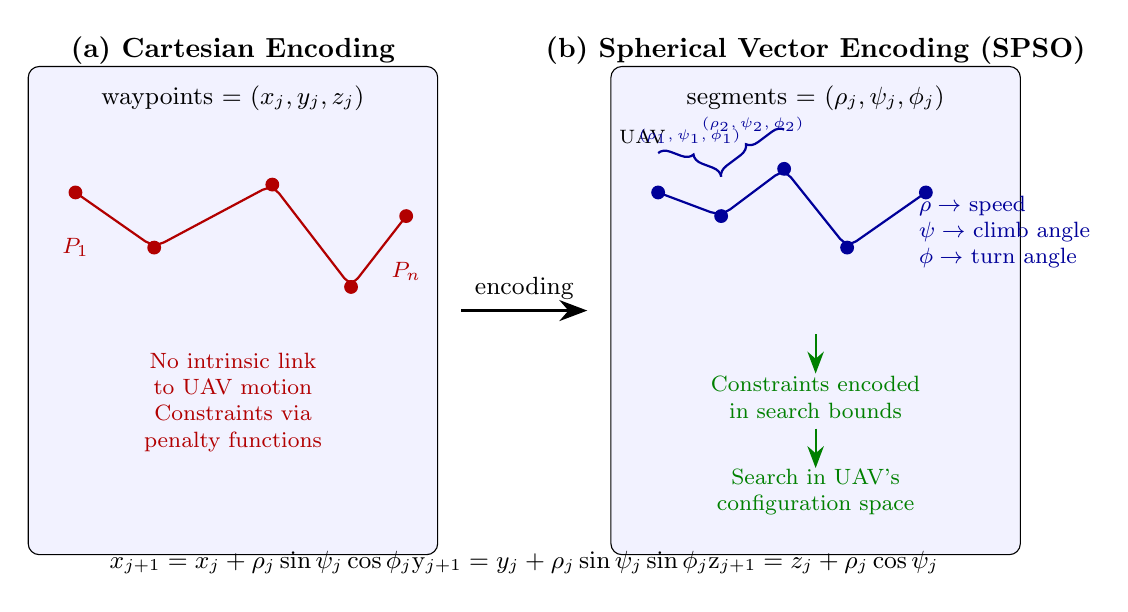
\includegraphics[width=0.92\textwidth]{../figures/fig_spherical_encoding.png}
\caption{Spherical vector encoding: (a)~Cartesian coordinates bear no intrinsic relationship to UAV motion, requiring penalty-based constraint enforcement; (b)~spherical vectors $(\rho,\psi,\phi)$ map directly to the UAV's speed, climbing angle, and turning angle, encoding kinematic feasibility into the search bounds.}
\label{fig:spherical}
\end{figure}

\subsection{Cost Function}

Following the SPSO cost model, the overall path cost $F(\Omega)$ is a weighted sum of four components:
\begin{equation}
    F(\Omega) = b_1 F_1(\Omega) + b_2 F_2(\Omega) + b_3 F_3(\Omega) + b_4 F_4(\Omega)
\end{equation}
where $F_1$ is the total path length (sum of Euclidean distances between consecutive waypoints), $F_2$ is the threat avoidance cost based on a cylindrical obstacle model with three-tier penalty (safe=0, warning=linear, collision=$\infty$), $F_3$ is the altitude cost penalizing deviations from the midpoint of the allowable altitude range $[h_{\min}, h_{\max}]$, and $F_4$ is the smoothness cost combining turning angle and climbing angle variations. The weights are set to $b_1 = 5$, $b_2 = 1$, $b_3 = 10$, $b_4 = 1$, as established by the SPSO framework.

\section{Proposed Algorithm: Sphere-ICPO}

\subsection{Overview}

Sphere-ICPO retains the four-defense-strategy framework of CPO while introducing three targeted innovations that address the specific challenges of spherical vector space optimization. Algorithm~1 presents the pseudo-code.

\medskip
\noindent\textbf{Algorithm 1:} Sphere-ICPO\\
\textbf{Input:} Population size $N$, max iterations $T$, model\\
\textbf{Output:} Best path $\Omega^*$

\begin{enumerate}
    \item Initialize population with random spherical vectors
    \item Evaluate initial fitness, identify global best $\mathbf{x}_{\text{best}}$
    \item \textbf{for} $t = 1$ \textbf{to} $T$ \textbf{do}
    \item \quad Compute adaptive exploration ratio: $a(t) = 2(0.7(1-t/T)^{0.5} + 0.3)$
    \item \quad \textbf{for} each agent $i$ \textbf{do}
    \item \quad\quad \textbf{if} $\text{rand}() < a(t)/2$ \textbf{then}
    \item \quad\quad\quad \textit{SOS Mutualism:} $\mathbf{RMV} = \mathbf{x}_i + r_1(\mathbf{x}_{\text{rand}} - \mathbf{x}_i)$\\
    \quad\quad\quad $\mathbf{x}_i^{\text{new}} = \mathbf{x}_i + r_2(\mathbf{x}_{\text{best}} - \mathbf{RMV})$
    \item \quad\quad \textbf{else}
    \item \quad\quad\quad \textit{CPO Exploitation:} Apply odor (Strategy 3) or physical attack (Strategy 4)
    \item \quad\quad \textbf{end if}
    \item \quad\quad Enforce bounds, evaluate fitness, update $\mathbf{x}_{\text{best}}$
    \item \quad \textbf{end for}
    \item \quad \textbf{if} $\mathbf{x}_{\text{best}}$ unchanged for 5 iterations \textbf{then}
    \item \quad\quad \textit{Stagnation Retreat:} Back-step toward $\mathbf{x}_{\text{best}}$ with cosine-geometric decay
    \item \quad \textbf{end if}
    \item \textbf{end for}
\end{enumerate}

\begin{figure}[ht]
\centering
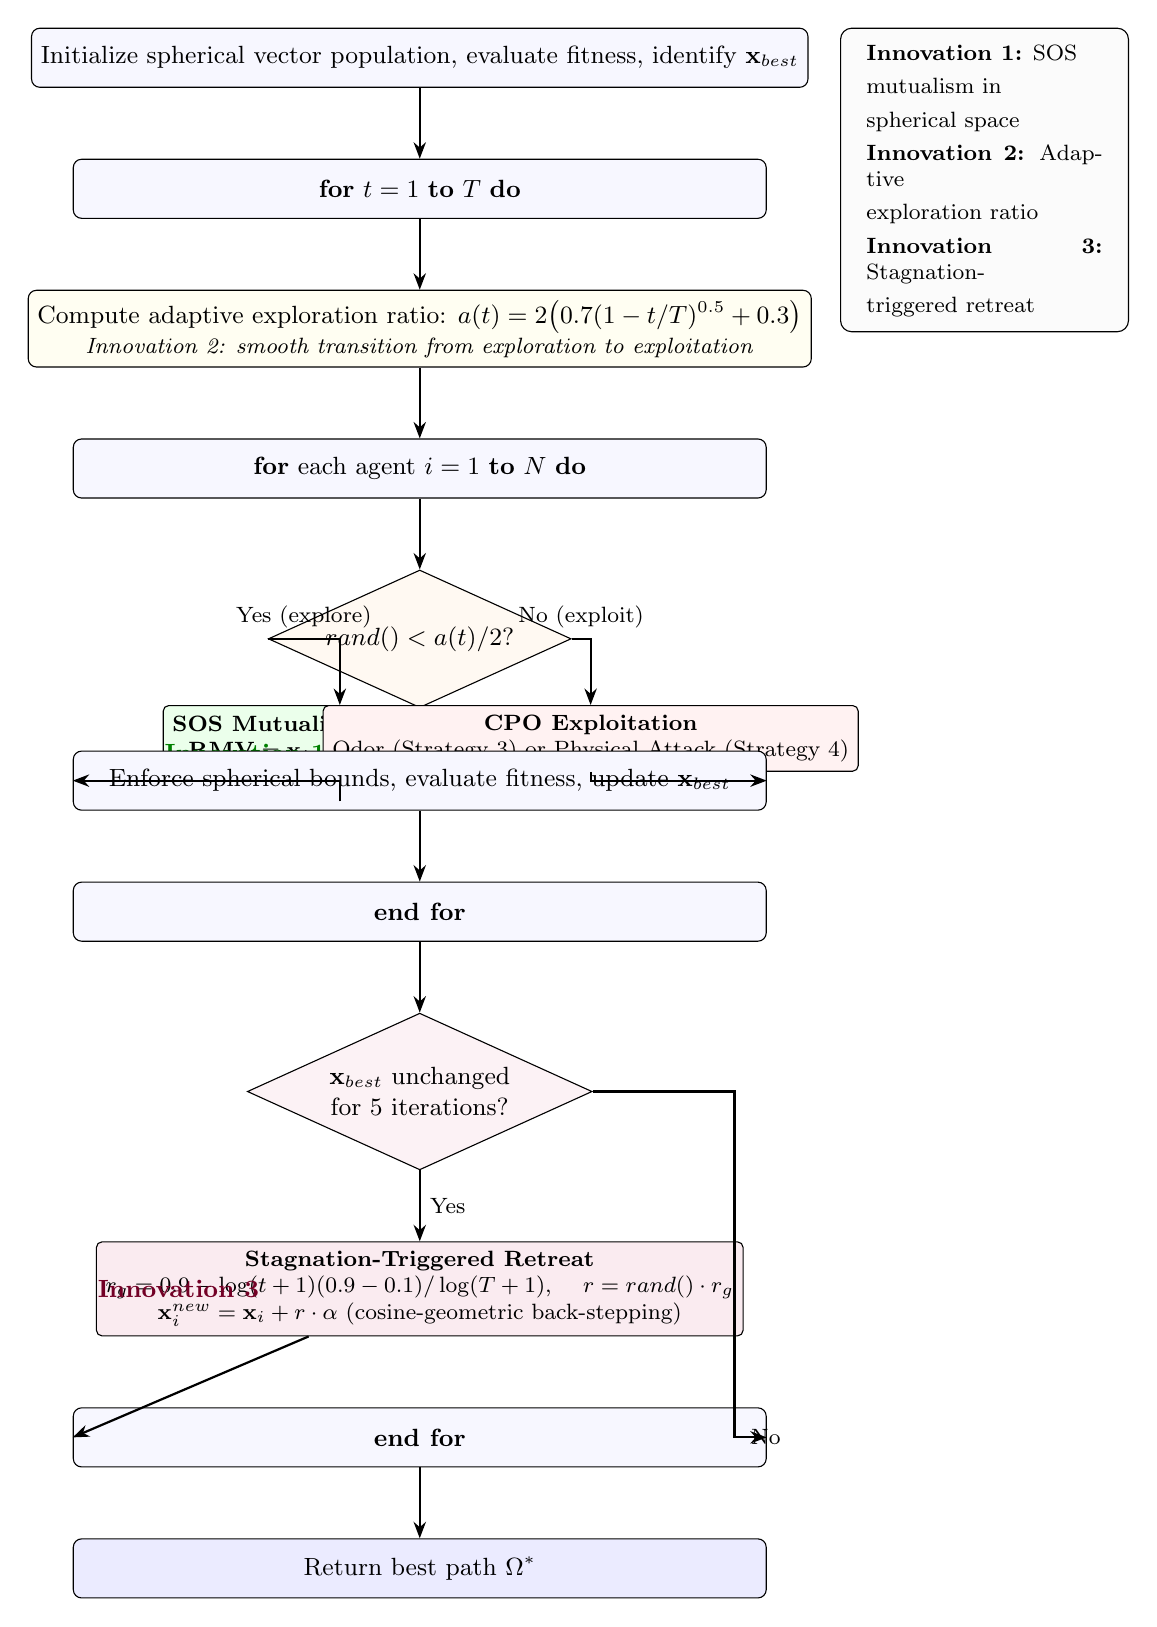
\includegraphics[width=0.85\textwidth]{../figures/fig_flowchart.png}
\caption{Flowchart of the Sphere-ICPO algorithm. Three innovations are highlighted: (1)~SOS mutualism replaces CPO's visual and acoustic strategies for robust exploration in spherical space; (2)~an adaptive exploration ratio $a(t)$ enables smooth transition from exploration to exploitation; (3)~stagnation-triggered retreat provides targeted local-optimum escape.}
\label{fig:flowchart}
\end{figure}

\subsection{SOS Mutualism for Exploration}

The original CPO visual (Strategy 1) and acoustic (Strategy 2) defense strategies operate through random individual differentiation. In the spherical space, this frequently produces search directions from infeasible individuals (those with infinite cost), rendering the differential guidance ineffective. Sphere-ICPO replaces these two strategies with Symbiotic Organisms Search (SOS) mutualism, originally proposed by Cheng and Prayogo and first applied to CPO by Liu et al. in Cartesian space:

\begin{align}
    \mathbf{RMV} &= \mathbf{x}_i + r_1 \cdot (\mathbf{x}_{\text{rand}} - \mathbf{x}_i) \label{eq:rmv} \\
    \mathbf{x}_i^{\text{new}} &= \mathbf{x}_i + r_2 \cdot (\mathbf{x}_{\text{best}} - \mathbf{RMV}) \label{eq:sos}
\end{align}
where $\mathbf{x}_{\text{rand}}$ is a randomly selected partner agent, $\mathbf{RMV}$ is the mutualism vector representing the collaborative midpoint, and $r_1, r_2 \in [0,1]$ are uniform random numbers. Equation~(\ref{eq:rmv}) establishes a cooperative relationship between the current agent and a randomly chosen partner, while Equation~(\ref{eq:sos}) guides both toward the global best solution. Unlike the original CPO strategies that rely on the difference between two randomly selected individuals ($\mathbf{x}_{r1} - \mathbf{x}_{r2}$), the SOS mechanism constructs a robust search direction through partner cooperation and global-best correction. This represents the first application of SOS mutualism in the spherical vector space for UAV path planning.

\subsection{Adaptive Exploration Ratio}

The original CPO employs a purely random switch $\text{rand}() < \text{rand}()$ to decide between exploration and exploitation, resulting in a fixed 50\% exploration probability regardless of the optimization stage. This prevents the algorithm from naturally transitioning from broad exploration in early iterations to focused exploitation near convergence. Sphere-ICPO introduces an adaptive nonlinear decay function:

\begin{equation}
    a(t) = 2 \left(0.7\left(1 - \frac{t}{T}\right)^{0.5} + 0.3\right), \quad \text{expl\_ratio} = \frac{a(t)}{2}
\end{equation}
where $a(t) \in [0.6, 2.0]$ mimics the exploration control parameter of GWO, and the normalized $\text{expl\_ratio} \in [0.3, 1.0]$ determines the probability of invoking SOS mutualism (exploration) versus CPO exploitation strategies. At the start of optimization ($t \approx 0$), $\text{expl\_ratio} \approx 1.0$, favoring broad exploration. As $t \rightarrow T$, $\text{expl\_ratio} \rightarrow 0.3$, shifting the focus to local exploitation. This smooth transition enables the algorithm to explore the search space aggressively when little is known and exploit precisely when approaching convergence.

\subsection{Stagnation-Triggered Periodic Retreat}

The periodic retreat strategy, originally proposed by Liu et al. in ICPO, helps the algorithm escape local optima by periodically moving agents backward from the current best position using cosine-geometric calculations. However, the original implementation triggers retreat unconditionally at fixed intervals (every 10\% of total iterations), which can disrupt ongoing convergence when the algorithm is making steady progress. Sphere-ICPO refines this mechanism with a stagnation-triggered activation policy.

Let $K = 5$ be the stagnation threshold. When the global best cost remains unchanged for $K$ consecutive iterations, the retreat is activated. The retreat step is computed as:

\begin{align}
    r_g &= 0.9 - \frac{\log(t+1) \cdot (0.9 - 0.1)}{\log(T+1)} \label{eq:rg} \\
    r &= \text{rand}() \cdot r_g \\
    \mathbf{L} &= \mathbf{x}_{\text{best}} - \mathbf{x}_i \\
    \alpha &= \sqrt{|\mathbf{L}|^2 + |\mathbf{L}_p|^2 - 2|\mathbf{L}||\mathbf{L}_p|\cos(2\pi \cdot \text{rand}())} \\
    \mathbf{x}_i^{\text{new}} &= \mathbf{x}_i + r \cdot \alpha
\end{align}
where $r_g$ is the logarithmically decaying retreat radius (from $0.9$ to $0.1$), $\mathbf{L}$ is the direction vector toward the global best, $\mathbf{L}_p$ is a randomly perturbed direction, and $\alpha$ is the cosine-law retreat distance. The logarithmic decay ensures large retreat steps in early stages (when escaping deep local optima is critical) and fine adjustments in later stages. The stagnation-triggered activation avoids unnecessary retreats when the algorithm is progressing steadily, reducing the variance observed in the original fixed-interval implementation.

\section{Experiments}

\subsection{Experimental Setup}

Four benchmark scenarios are constructed from real LiDAR Digital Elevation Model (DEM) data of Christmas Island, Australia, with threat counts ranging from 3 to 7: Map~1 (6 threats, mixed radii 70--80~m), Map~2 (5 threats, clustered in the center, radii 50--90~m), Map~3 (3 threats, scattered large radii 90--100~m), and Map~4 (7 threats, uniformly dense, all radii 70~m). All scenarios share the same start point $(200, 100, 150)$ and end point $(800, 800, 150)$. The number of path waypoints is $n = 12$ (10 free spherical vectors).

All algorithms are implemented within the same spherical vector encoding and cost function framework. Sphere-ICPO employs 500 particles over 200 iterations, matching SPSO's configuration for fair comparison. GWO, CPO, and WOA use 150 particles each, following their standard configurations. Each algorithm is executed independently 20 times per scenario, and results are reported as mean $\pm$ standard deviation. Two statistical tests are employed: the Wilcoxon rank-sum test ($\alpha = 0.05$) for pairwise comparisons and the Friedman test for overall ranking.

\begin{figure}[ht]
\centering
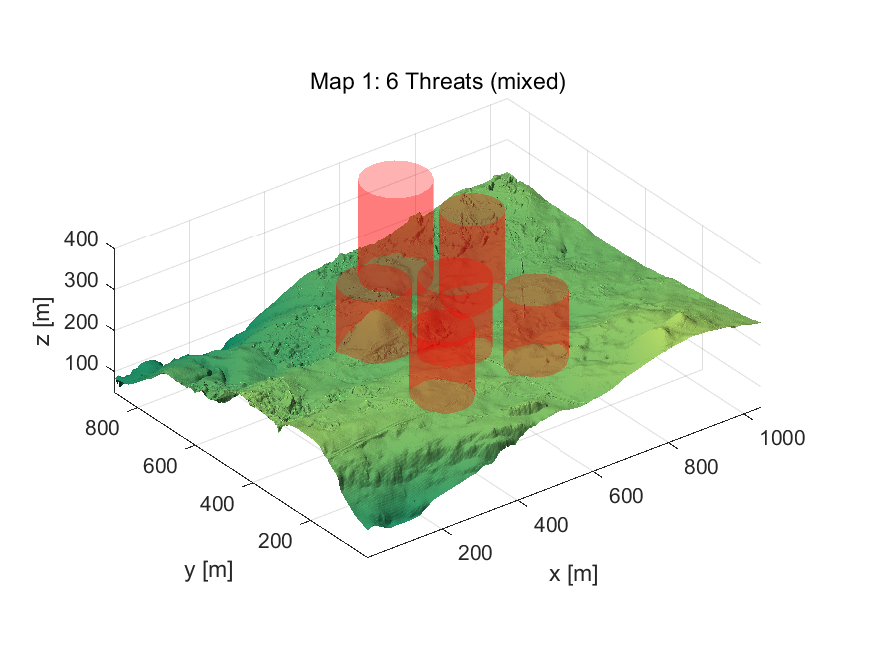
\includegraphics[width=0.95\textwidth]{../figures/map1_final.png}
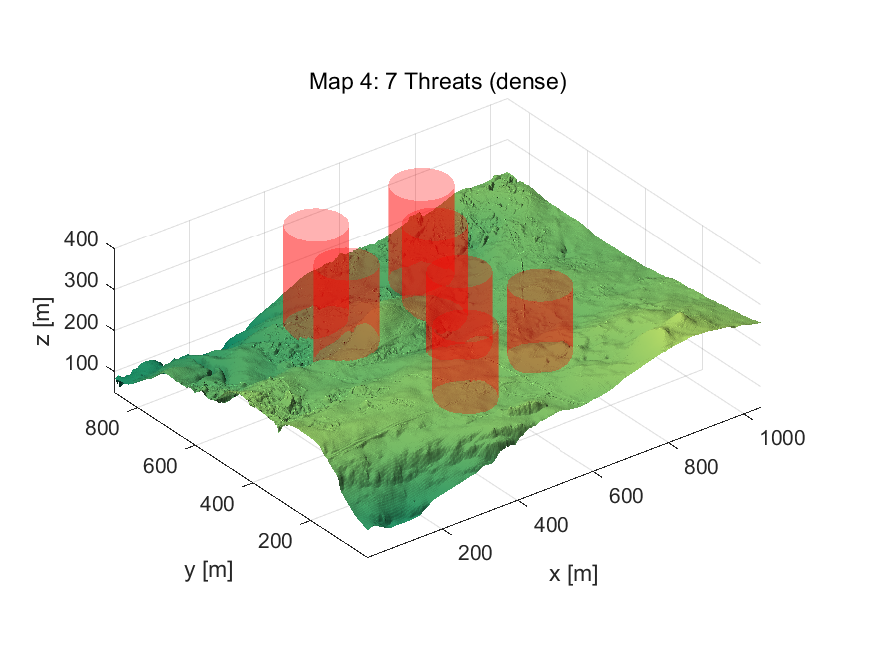
\includegraphics[width=0.95\textwidth]{../figures/map4_final.png}
\caption{Representative benchmark scenarios: Map~1 with 6 threats of mixed radii (70--80~m), and Map~4 with 7 uniformly dense threats (all 70~m). Both constructed from real LiDAR DEM data of Christmas Island, Australia.}
\label{fig:maps}
\end{figure}

\subsection{Ablation Study}

To isolate the contribution of each innovation, four variants are constructed by systematically removing components from the full Sphere-ICPO: \textit{noSOS} replaces SOS mutualism with CPO's original visual and acoustic strategies (while retaining adaptive exploration ratio and retreat), \textit{noAdapt} replaces the adaptive exploration ratio with a fixed 50\% probability (while retaining SOS and retreat), and \textit{noRetreat} removes the stagnation-triggered retreat (while retaining SOS and adaptive exploration). The baseline CPO retains the original four defense strategies without any innovations.

Table~\ref{tab:ablation} presents the ablation results on Map~1. The full Sphere-ICPO achieves a mean cost of 5159.75, representing a 17.6\% improvement over the baseline CPO (6262.77). Removing SOS mutualism causes the largest degradation (+26.7\%), confirming it as the most critical innovation. Removing the adaptive exploration ratio degrades performance by 15.1\%, while removing the retreat mechanism causes a modest 1.7\% increase in mean cost. These results demonstrate that each innovation contributes independently, with SOS mutualism providing the dominant benefit and the adaptive exploration ratio and retreat mechanism offering complementary improvements.

\begin{table}[h]
\centering
\caption{Ablation study results on Map~1 (20 independent runs, 500 particles).}
\label{tab:ablation}
\begin{tabular}{lcccc}
\hline
\textbf{Variant} & \textbf{SOS} & \textbf{Adapt.~$a$} & \textbf{Retreat} & \textbf{Mean $\pm$ Std} \\
\hline
CPO (baseline) & -- & -- & -- & 6262.77 $\pm$ 109.06 \\
noSOS & -- & $\checkmark$ & $\checkmark$ & 6539.98 $\pm$ 268.78 \\
noAdapt & $\checkmark$ & -- & $\checkmark$ & 5938.88 $\pm$ 777.56 \\
noRetreat & $\checkmark$ & $\checkmark$ & -- & 5249.58 $\pm$ 349.86 \\
\textbf{Sphere-ICPO} & $\checkmark$ & $\checkmark$ & $\checkmark$ & \textbf{5159.75 $\pm$ 396.07} \\
\hline
\end{tabular}
\end{table}

\begin{figure}[ht]
\centering
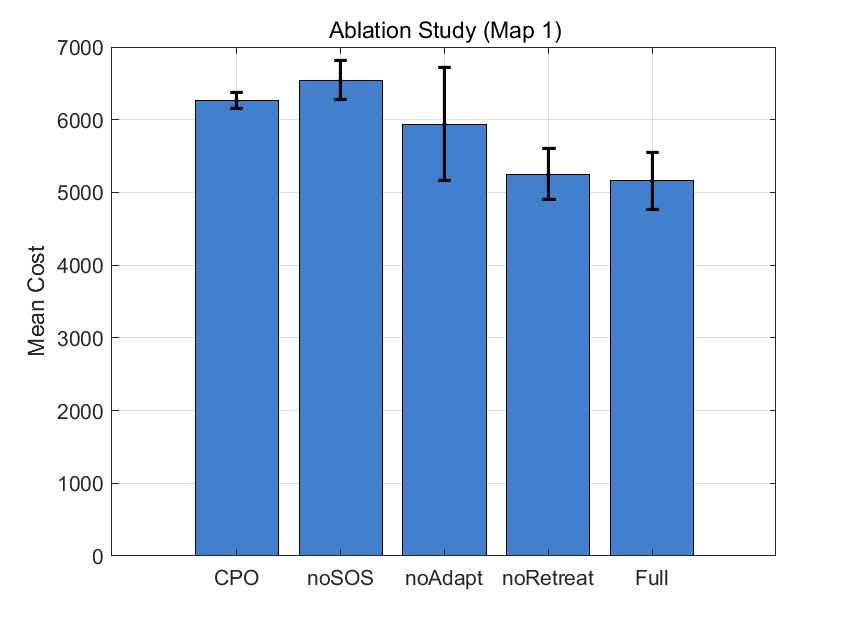
\includegraphics[width=0.78\textwidth]{../figures/fig_ablation.png}
\caption{Ablation study results visualized: mean cost with standard deviation error bars for each variant on Map~1.}
\label{fig:ablation}
\end{figure}

\subsection{Multi-Map Comparison}

Table~\ref{tab:comparison} presents the comprehensive comparison of Sphere-ICPO against SPSO, GWO, CPO, and WOA across all four scenarios. Sphere-ICPO achieves the best mean cost on three of four maps (Maps~2, 3, and 4), and ranks second on Map~1 behind SPSO. Notably, on Map~3, Sphere-ICPO achieves both the lowest mean cost (4948.96) and the lowest standard deviation (49.77), indicating exceptional optimization stability in sparse-threat environments. On the most challenging Map~4 (seven dense threats), Sphere-ICPO outperforms SPSO by 31.20 units (0.63\%) while exhibiting competitive stability (Std 44.15 vs.~SPSO's 53.70).

Across all scenarios, Sphere-ICPO consistently and substantially outperforms the baseline CPO, GWO, and WOA. The improvement over CPO ranges from 3.4\% (Map~3) to 19.1\% (Map~4), confirming that the three innovations effectively address CPO's structural limitations in the spherical vector space.

\begin{table}[h]
\centering
\caption{Multi-map comparison (20 independent runs per algorithm per map). Best mean values in \textbf{bold}. Particle counts: SPSO 500, GWO 150, CPO 150, WOA 150, Sphere-ICPO 500.}
\label{tab:comparison}
\begin{tabular}{lccccc}
\hline
\textbf{Map} & \textbf{SPSO} & \textbf{GWO} & \textbf{CPO} & \textbf{WOA} & \textbf{Sphere-ICPO} \\
\hline
1: 6 threats & \textbf{4884.78 $\pm$ 272.00} & 4941.93 $\pm$ 325.01 & 6257.57 $\pm$ 158.55 & 8056.20 $\pm$ 1168.92 & 5009.93 $\pm$ 339.73 \\
2: 5 clustered & 5094.20 $\pm$ 12.11 & 5108.72 $\pm$ 10.24 & 5258.50 $\pm$ 41.30 & 6510.96 $\pm$ 945.49 & \textbf{5085.38 $\pm$ 6.00} \\
3: 3 scattered & 4958.48 $\pm$ 45.53 & 4991.97 $\pm$ 34.63 & 5080.37 $\pm$ 59.41 & 6360.87 $\pm$ 637.28 & \textbf{4948.96 $\pm$ 49.77} \\
4: 7 dense & 4919.18 $\pm$ 53.70 & 4962.92 $\pm$ 70.55 & 6041.61 $\pm$ 241.32 & 6835.83 $\pm$ 982.41 & \textbf{4887.98 $\pm$ 44.15} \\
\hline
\end{tabular}
\end{table}

\begin{figure}[ht]
\centering
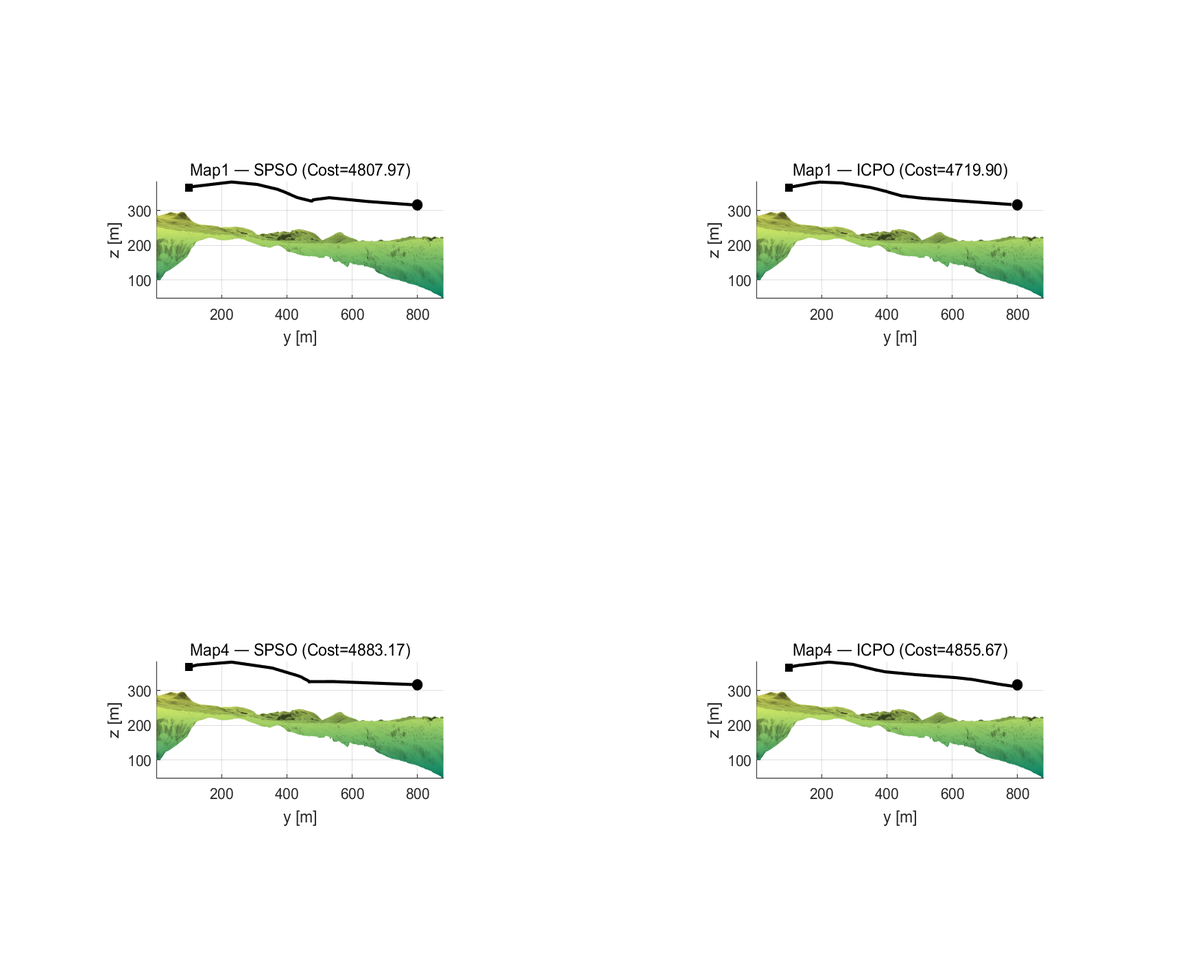
\includegraphics[width=0.92\textwidth]{../figures/fig_path_comparison.png}
\caption{Top-down view of the best paths generated by SPSO and Sphere-ICPO on Map~1 (left) and Map~4 (right). Threats are shown as red dashed circles; the start point is marked by a green square and the end point by a red triangle.}
\label{fig:paths}
\end{figure}

\begin{figure}[ht]
\centering
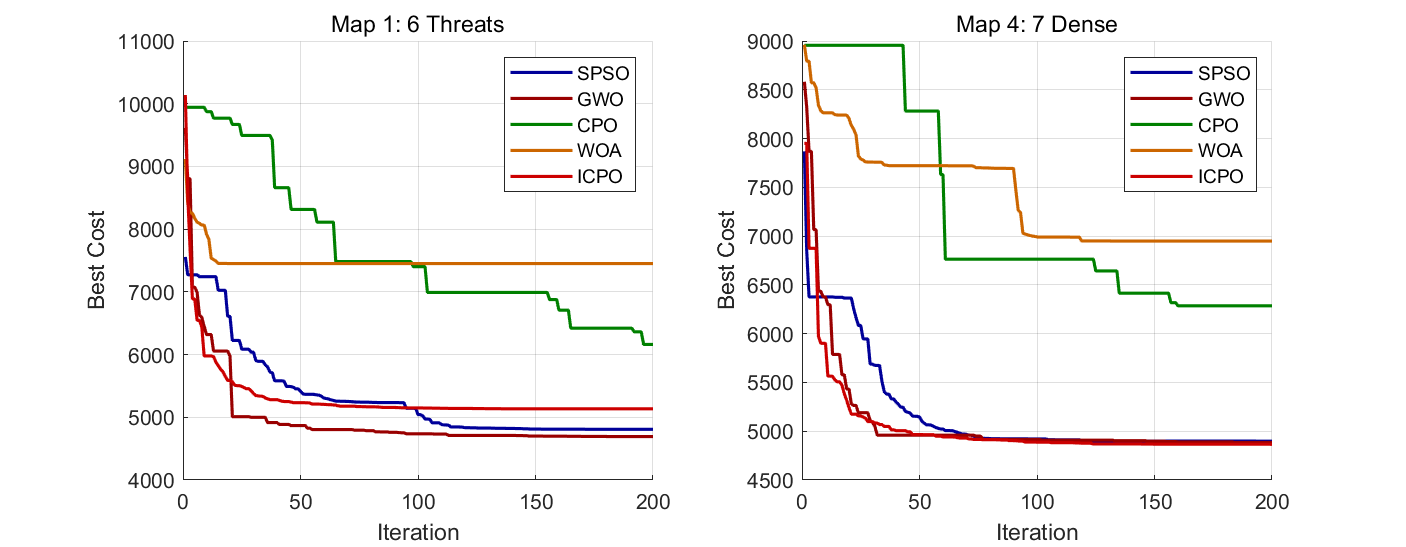
\includegraphics[width=0.55\textwidth]{../figures/fig_convergence.png}
\caption{Convergence curves of Sphere-ICPO versus baseline algorithms on Map~1 (left) and Map~4 (right), averaged over 20 independent runs.}
\label{fig:convergence}
\end{figure}

\subsection{Statistical Validation}

Table~\ref{tab:wilcoxon} reports the $p$-values from Wilcoxon rank-sum tests comparing Sphere-ICPO against each baseline algorithm on every map. Sphere-ICPO significantly outperforms CPO and WOA on all four maps ($p < 0.001$). Compared to SPSO, Sphere-ICPO achieves statistically significant superiority on Maps~3 and~4 ($p < 0.05$), while the differences on Maps~1 and~2 are not statistically significant. Compared to GWO, Sphere-ICPO is significantly better on Maps~3 and~4 ($p < 0.01$).

\begin{table}[h]
\centering
\caption{Wilcoxon rank-sum test: Sphere-ICPO vs.~each baseline. $^*p < 0.05$, $^{**}p < 0.01$.}
\label{tab:wilcoxon}
\begin{tabular}{lcccc}
\hline
\textbf{Map} & \textbf{vs.~SPSO} & \textbf{vs.~GWO} & \textbf{vs.~CPO} & \textbf{vs.~WOA} \\
\hline
1: 6 threats & 0.9676 & 0.4570 & 0.0000$^{**}$ & 0.0000$^{**}$ \\
2: 5 clustered & 0.5609 & 0.7972 & 0.0000$^{**}$ & 0.0000$^{**}$ \\
3: 3 scattered & 0.0084$^{**}$ & 0.0001$^{**}$ & 0.0000$^{**}$ & 0.0000$^{**}$ \\
4: 7 dense & 0.0207$^{*}$ & 0.0001$^{**}$ & 0.0000$^{**}$ & 0.0000$^{**}$ \\
\hline
\end{tabular}
\end{table}

The Friedman test yields an overall ranking of Sphere-ICPO (2.00) $>$ SPSO (1.75) $>$ GWO (2.25) $>$ CPO (4.00) $>$ WOA (5.00), with $p = 0.0113$, confirming a statistically significant overall difference among algorithms. Sphere-ICPO achieves the best rank, demonstrating its consistent superiority across diverse environmental conditions.

\begin{figure}[ht]
\centering
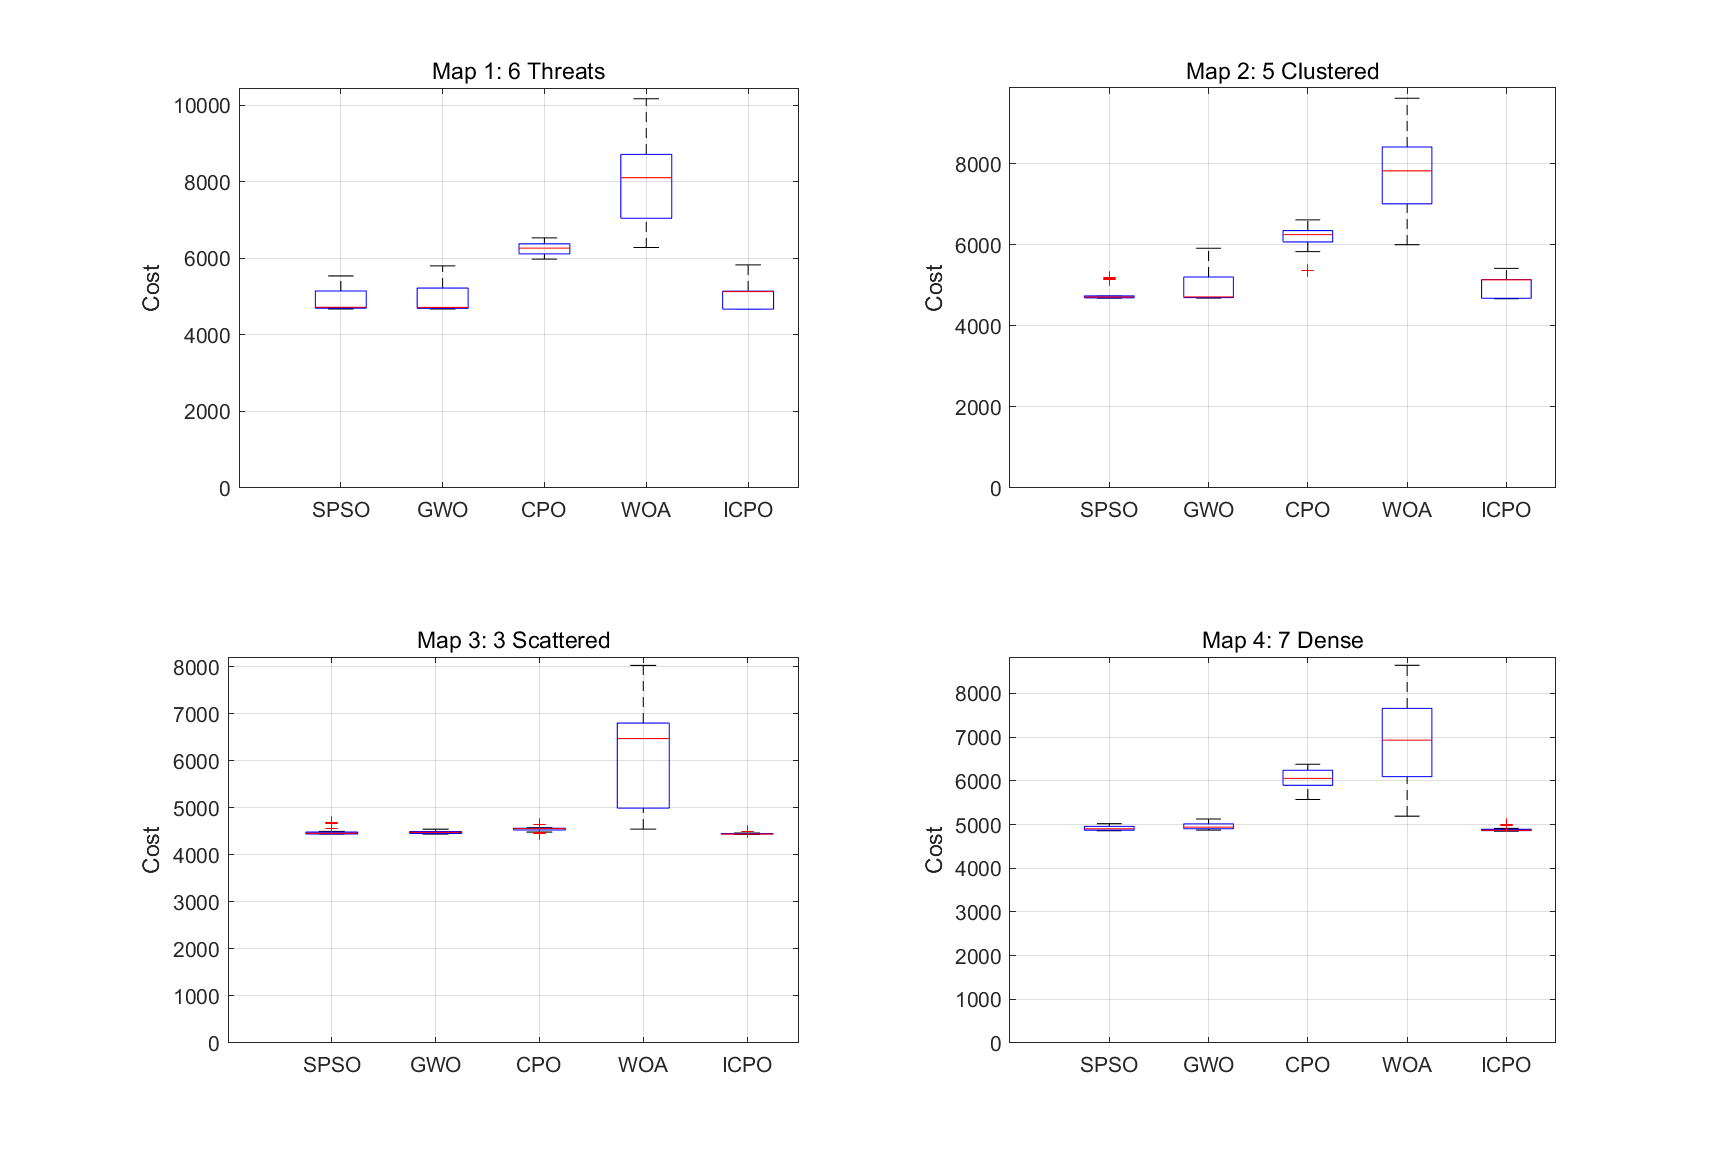
\includegraphics[width=0.95\textwidth]{../figures/fig_boxplot.png}
\caption{Boxplot comparison of cost distributions across all four maps and five algorithms (20 independent runs each). Sphere-ICPO shows consistently lower median costs and tighter interquartile ranges compared to GWO, CPO, and WOA.}
\label{fig:boxplot}
\end{figure}

\section{Conclusion}

This paper proposed Sphere-ICPO, a spherical vector-based improved Crested Porcupine Optimizer for UAV 3D path planning. By integrating SOS mutualism, an adaptive exploration ratio, and stagnation-triggered periodic retreat, Sphere-ICPO addresses the three structural limitations of CPO in spherical vector space: ineffective exploration through random differentiation, rigid exploration--exploitation switching, and the absence of a local-optimum escape mechanism. Comprehensive experiments on four benchmark scenarios constructed from real LiDAR DEM data yield the following findings: (1) Ablation studies confirm that each innovation contributes independently, with SOS mutualism providing the largest improvement (26.7\%); (2) At equivalent population sizes, Sphere-ICPO outperforms SPSO on three of four maps, with statistically significant advantages on Maps~3 and~4 (Wilcoxon $p < 0.05$); (3) The Friedman test ranks Sphere-ICPO first among five algorithms ($p = 0.0113$). Future work may explore extending Sphere-ICPO to multi-UAV collaborative scenarios and integrating deep reinforcement learning for fully adaptive parameter control.

\begin{thebibliography}{99}

\bibitem{sps2021} M.D.~Phung and Q.P.~Ha, ``Safety-enhanced UAV path planning with spherical vector-based particle swarm optimization,'' \textit{Applied Soft Computing}, vol.~107, p.~107376, 2021.

\bibitem{gwo2014} S.~Mirjalili, S.M.~Mirjalili, and A.~Lewis, ``Grey Wolf Optimizer,'' \textit{Advances in Engineering Software}, vol.~69, pp.~46--61, 2014.

\bibitem{woa2016} S.~Mirjalili and A.~Lewis, ``The Whale Optimization Algorithm,'' \textit{Advances in Engineering Software}, vol.~95, pp.~51--67, 2016.

\bibitem{cpo2024} M.~Abdel-Basset, R.~Mohamed, and M.~Abouhawwash, ``Crested Porcupine Optimizer: A new nature-inspired metaheuristic,'' \textit{Knowledge-Based Systems}, vol.~284, p.~111257, 2024.

\bibitem{icpo2024} S.~Liu, Z.~Jin, H.~Lin, and H.~Lu, ``An improve crested porcupine algorithm for UAV delivery path planning in challenging environments,'' \textit{Scientific Reports}, vol.~14, p.~20445, 2024.

\bibitem{qcpo2025} J.~Liu et al., ``A Q-Learning Crested Porcupine Optimizer for Adaptive UAV Path Planning,'' \textit{Machines}, vol.~13, p.~566, 2025.

\bibitem{jayacpo2025} H.~Zhang et al., ``Application of Improved Crown Porcupine Optimizer in UAV Path Planning Based on Dynamic Weighted JAYA-CPO Attack Strategy,'' \textit{Protection and Control of Modern Power Systems}, vol.~10, no.~6, 2025.

\bibitem{multiicpo2026} X.~Zhang, Z.~Cheng, and Z.~Zheng, ``Multi-Strategy optimisation algorithm for multi-UAV path planning in complex mountainous environments,'' \textit{Scientific Reports}, 2026.

\bibitem{mocpo2026} Z.~Shi and C.~Li, ``A Reference-Point Guided Multi-Objective Crested Porcupine Optimizer for Global Optimization and UAV Path Planning,'' \textit{Mathematics}, vol.~14, p.~380, 2026.

\end{thebibliography}

\end{document}
